\documentclass[1p]{elsarticle_modified}
%\bibliographystyle{elsarticle-num}

%\usepackage[colorlinks]{hyperref}
%\usepackage{abbrmath_seonhwa} %\Abb, \Ascr, \Acal ,\Abf, \Afrak
\usepackage{amsfonts}
\usepackage{amssymb}
\usepackage{amsmath}
\usepackage{amsthm}
\usepackage{scalefnt}
\usepackage{amsbsy}
\usepackage{kotex}
\usepackage{caption}
\usepackage{subfig}
\usepackage{color}
\usepackage{graphicx}
\usepackage{xcolor} %% white, black, red, green, blue, cyan, magenta, yellow
\usepackage{float}
\usepackage{setspace}
\usepackage{hyperref}

\usepackage{tikz}
\usetikzlibrary{arrows}

\usepackage{multirow}
\usepackage{array} % fixed length table
\usepackage{hhline}

%%%%%%%%%%%%%%%%%%%%%
\makeatletter
\renewcommand*\env@matrix[1][\arraystretch]{%
	\edef\arraystretch{#1}%
	\hskip -\arraycolsep
	\let\@ifnextchar\new@ifnextchar
	\array{*\c@MaxMatrixCols c}}
\makeatother %https://tex.stackexchange.com/questions/14071/how-can-i-increase-the-line-spacing-in-a-matrix
%%%%%%%%%%%%%%%

\usepackage[normalem]{ulem}

\newcommand{\msout}[1]{\ifmmode\text{\sout{\ensuremath{#1}}}\else\sout{#1}\fi}
%SOURCE: \msout is \stkout macro in https://tex.stackexchange.com/questions/20609/strikeout-in-math-mode

\newcommand{\cancel}[1]{
	\ifmmode
	{\color{red}\msout{#1}}
	\else
	{\color{red}\sout{#1}}
	\fi
}

\newcommand{\add}[1]{
	{\color{blue}\uwave{#1}}
}

\newcommand{\replace}[2]{
	\ifmmode
	{\color{red}\msout{#1}}{\color{blue}\uwave{#2}}
	\else
	{\color{red}\sout{#1}}{\color{blue}\uwave{#2}}
	\fi
}

\newcommand{\Sol}{\mathcal{S}} %segment
\newcommand{\D}{D} %diagram
\newcommand{\A}{\mathcal{A}} %arc


%%%%%%%%%%%%%%%%%%%%%%%%%%%%%5 test

\def\sl{\operatorname{\textup{SL}}(2,\Cbb)}
\def\psl{\operatorname{\textup{PSL}}(2,\Cbb)}
\def\quan{\mkern 1mu \triangleright \mkern 1mu}

\theoremstyle{definition}
\newtheorem{thm}{Theorem}[section]
\newtheorem{prop}[thm]{Proposition}
\newtheorem{lem}[thm]{Lemma}
\newtheorem{ques}[thm]{Question}
\newtheorem{cor}[thm]{Corollary}
\newtheorem{defn}[thm]{Definition}
\newtheorem{exam}[thm]{Example}
\newtheorem{rmk}[thm]{Remark}
\newtheorem{alg}[thm]{Algorithm}

\newcommand{\I}{\sqrt{-1}}
\begin{document}

%\begin{frontmatter}
%
%\title{Boundary parabolic representations of knots up to 8 crossings}
%
%%% Group authors per affiliation:
%\author{Yunhi Cho} 
%\address{Department of Mathematics, University of Seoul, Seoul, Korea}
%\ead{yhcho@uos.ac.kr}
%
%
%\author{Seonhwa Kim} %\fnref{s_kim}}
%\address{Center for Geometry and Physics, Institute for Basic Science, Pohang, 37673, Korea}
%\ead{ryeona17@ibs.re.kr}
%
%\author{Hyuk Kim}
%\address{Department of Mathematical Sciences, Seoul National University, Seoul 08826, Korea}
%\ead{hyukkim@snu.ac.kr}
%
%\author{Seokbeom Yoon}
%\address{Department of Mathematical Sciences, Seoul National University, Seoul, 08826,  Korea}
%\ead{sbyoon15@snu.ac.kr}
%
%\begin{abstract}
%We find all boundary parabolic representation of knots up to 8 crossings.
%
%\end{abstract}
%\begin{keyword}
%    \MSC[2010] 57M25 
%\end{keyword}
%
%\end{frontmatter}

%\linenumbers
%\tableofcontents
%
\newcommand\colored[1]{\textcolor{white}{\rule[-0.35ex]{0.8em}{1.4ex}}\kern-0.8em\color{red} #1}%
%\newcommand\colored[1]{\textcolor{white}{ #1}\kern-2.17ex	\textcolor{white}{ #1}\kern-1.81ex	\textcolor{white}{ #1}\kern-2.15ex\color{red}#1	}

{\Large $\underline{12a_{1151}~(K12a_{1151})}$}

\setlength{\tabcolsep}{10pt}
\renewcommand{\arraystretch}{1.6}
\vspace{1cm}\begin{tabular}{m{100pt}>{\centering\arraybackslash}m{274pt}}
\multirow{5}{120pt}{
	\centering
	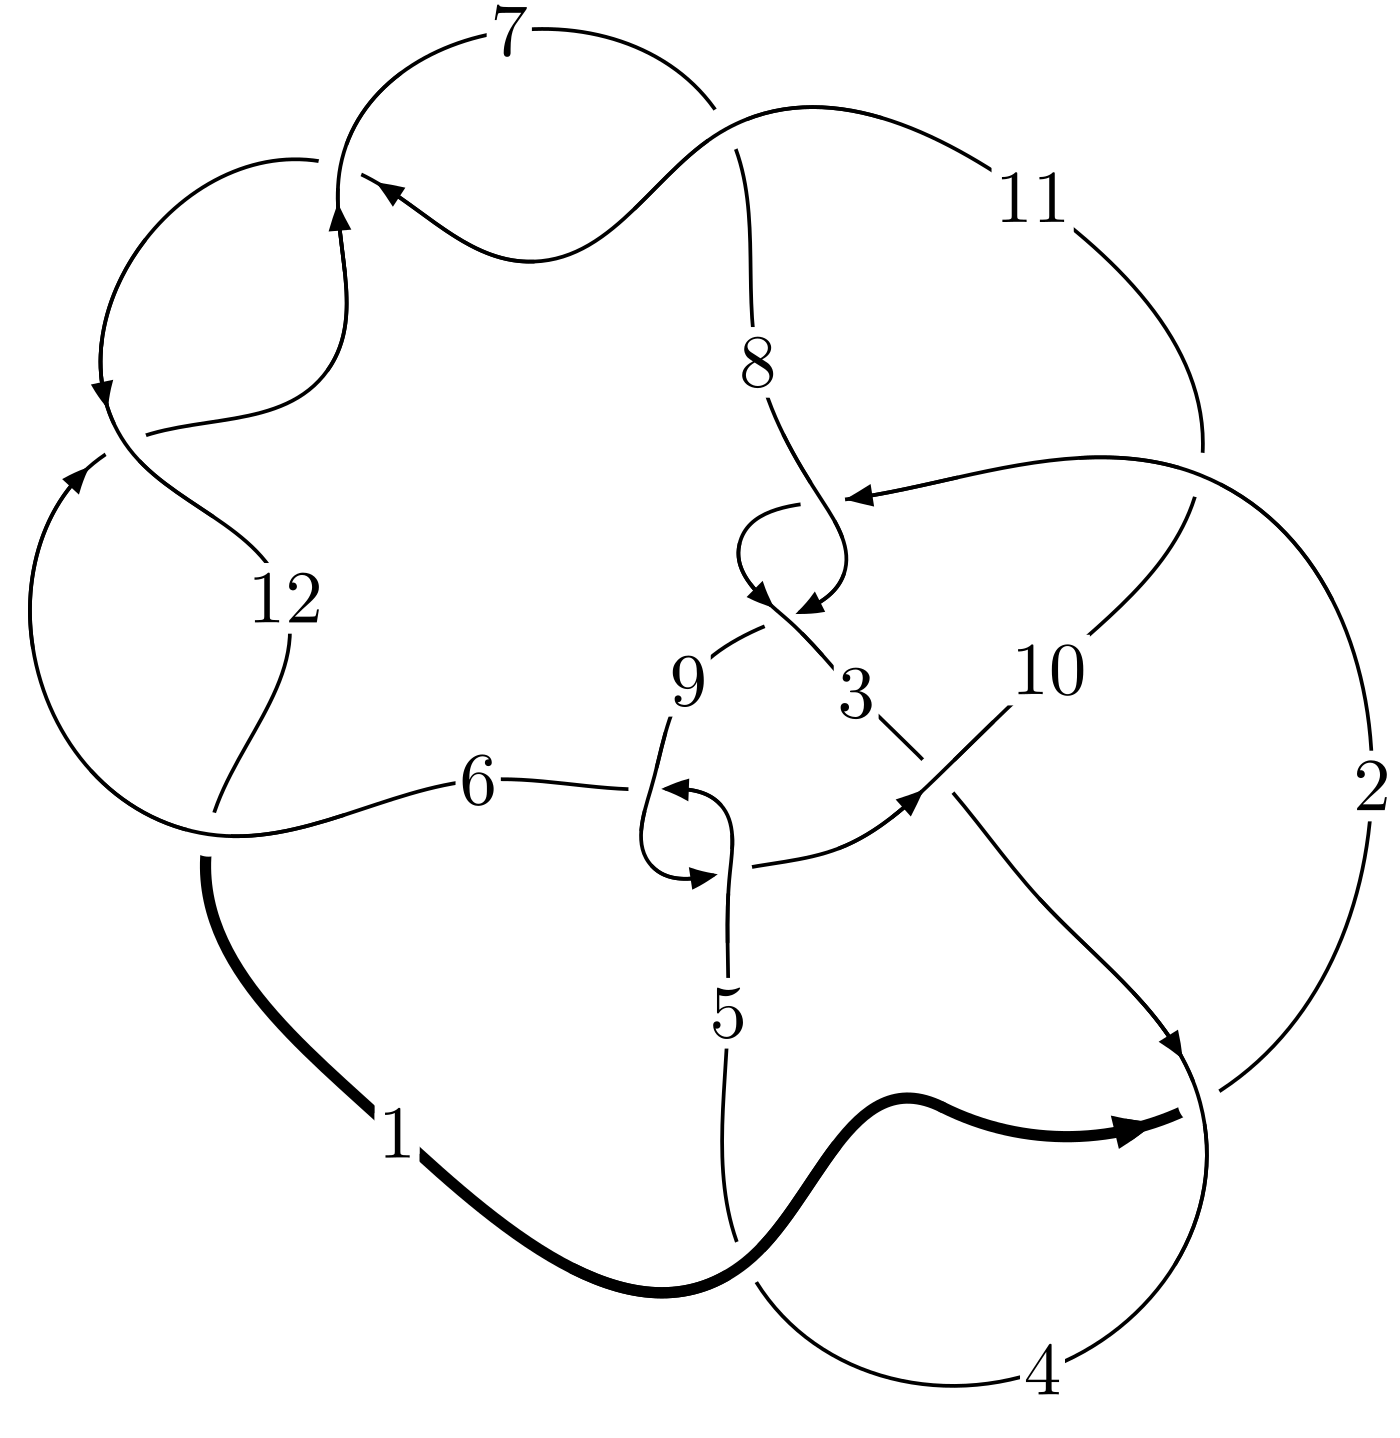
\includegraphics[width=112pt]{../../../GIT/diagram.site/Diagrams/png/1952_12a_1151.png}\\
\ \ \ A knot diagram\footnotemark}&
\allowdisplaybreaks
\textbf{Linearized knot diagam} \\
\cline{2-2}
 &
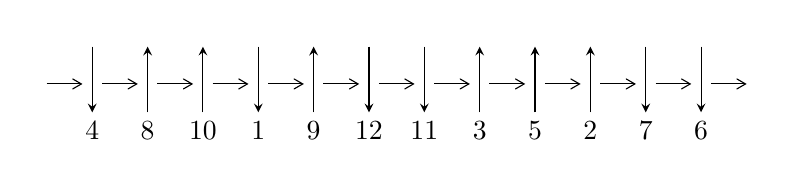
\begin{tikzpicture}[x=20pt, y=17pt]
	% nodes
	\node (C0) at (0, 0) {};
	\node (C1) at (1, 0) {};
	\node (C1U) at (1, +1) {};
	\node (C1D) at (1, -1) {4};

	\node (C2) at (2, 0) {};
	\node (C2U) at (2, +1) {};
	\node (C2D) at (2, -1) {8};

	\node (C3) at (3, 0) {};
	\node (C3U) at (3, +1) {};
	\node (C3D) at (3, -1) {10};

	\node (C4) at (4, 0) {};
	\node (C4U) at (4, +1) {};
	\node (C4D) at (4, -1) {1};

	\node (C5) at (5, 0) {};
	\node (C5U) at (5, +1) {};
	\node (C5D) at (5, -1) {9};

	\node (C6) at (6, 0) {};
	\node (C6U) at (6, +1) {};
	\node (C6D) at (6, -1) {12};

	\node (C7) at (7, 0) {};
	\node (C7U) at (7, +1) {};
	\node (C7D) at (7, -1) {11};

	\node (C8) at (8, 0) {};
	\node (C8U) at (8, +1) {};
	\node (C8D) at (8, -1) {3};

	\node (C9) at (9, 0) {};
	\node (C9U) at (9, +1) {};
	\node (C9D) at (9, -1) {5};

	\node (C10) at (10, 0) {};
	\node (C10U) at (10, +1) {};
	\node (C10D) at (10, -1) {2};

	\node (C11) at (11, 0) {};
	\node (C11U) at (11, +1) {};
	\node (C11D) at (11, -1) {7};

	\node (C12) at (12, 0) {};
	\node (C12U) at (12, +1) {};
	\node (C12D) at (12, -1) {6};
	\node (C13) at (13, 0) {};

	% arrows
	\draw[->,>={angle 60}]
	(C0) edge (C1) (C1) edge (C2) (C2) edge (C3) (C3) edge (C4) (C4) edge (C5) (C5) edge (C6) (C6) edge (C7) (C7) edge (C8) (C8) edge (C9) (C9) edge (C10) (C10) edge (C11) (C11) edge (C12) (C12) edge (C13) ;	\draw[->,>=stealth]
	(C1U) edge (C1D) (C2D) edge (C2U) (C3D) edge (C3U) (C4U) edge (C4D) (C5D) edge (C5U) (C6U) edge (C6D) (C7U) edge (C7D) (C8D) edge (C8U) (C9D) edge (C9U) (C10D) edge (C10U) (C11U) edge (C11D) (C12U) edge (C12D) ;
	\end{tikzpicture} \\
\hhline{~~} \\& 
\textbf{Solving Sequence} \\ \cline{2-2} 
 &
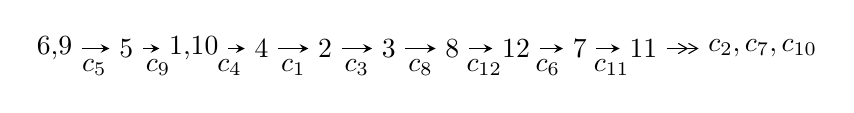
\begin{tikzpicture}[x=23pt, y=7pt]
	% node
	\node (A0) at (-1/8, 0) {6,9};
	\node (A1) at (1, 0) {5};
	\node (A2) at (33/16, 0) {1,10};
	\node (A3) at (25/8, 0) {4};
	\node (A4) at (33/8, 0) {2};
	\node (A5) at (41/8, 0) {3};
	\node (A6) at (49/8, 0) {8};
	\node (A7) at (57/8, 0) {12};
	\node (A8) at (65/8, 0) {7};
	\node (A9) at (73/8, 0) {11};
	\node (C1) at (1/2, -1) {$c_{5}$};
	\node (C2) at (3/2, -1) {$c_{9}$};
	\node (C3) at (21/8, -1) {$c_{4}$};
	\node (C4) at (29/8, -1) {$c_{1}$};
	\node (C5) at (37/8, -1) {$c_{3}$};
	\node (C6) at (45/8, -1) {$c_{8}$};
	\node (C7) at (53/8, -1) {$c_{12}$};
	\node (C8) at (61/8, -1) {$c_{6}$};
	\node (C9) at (69/8, -1) {$c_{11}$};
	\node (A10) at (11, 0) {$c_{2},c_{7},c_{10}$};

	% edge
	\draw[->,>=stealth]	
	(A0) edge (A1) (A1) edge (A2) (A2) edge (A3) (A3) edge (A4) (A4) edge (A5) (A5) edge (A6) (A6) edge (A7) (A7) edge (A8) (A8) edge (A9) ;
	\draw[->>,>={angle 60}]	
	(A9) edge (A10);
\end{tikzpicture} \\ 

\end{tabular} \\

\footnotetext{
The image of knot diagram is generated by the software ``\textbf{Draw programme}" developed by Andrew Bartholomew(\url{http://www.layer8.co.uk/maths/draw/index.htm\#Running-draw}), where we modified some parts for our purpose(\url{https://github.com/CATsTAILs/LinksPainter}).
}\phantom \\ \newline 
\centering \textbf{Ideals for irreducible components\footnotemark of $X_{\text{par}}$} 
 
\begin{align*}
I^u_{1}&=\langle 
-7.84155\times10^{139} u^{78}-5.86060\times10^{140} u^{77}+\cdots+3.54905\times10^{139} b+7.76498\times10^{140},\\
\phantom{I^u_{1}}&\phantom{= \langle  }-3.04871\times10^{140} u^{78}-2.59985\times10^{141} u^{77}+\cdots+3.54905\times10^{139} a-8.26678\times10^{141},\\
\phantom{I^u_{1}}&\phantom{= \langle  }u^{79}+9 u^{78}+\cdots+312 u+16\rangle \\
I^u_{2}&=\langle 
1422881983 u^{23}-5915588584 u^{22}+\cdots+1616424857 b-14740278204,\\
\phantom{I^u_{2}}&\phantom{= \langle  }629416068 u^{23}-2394813871 u^{22}+\cdots+1616424857 a+1027469093,\;u^{24}-2 u^{23}+\cdots+12 u^2+1\rangle \\
I^u_{3}&=\langle 
a^5 u- a^5+a^4-6 a^3 u+5 a^3+a^2 u-3 a^2+5 a u+3 b-6 a+4 u-4,\\
\phantom{I^u_{3}}&\phantom{= \langle  }a^6-6 a^4-3 a^3 u+3 a^2 u+9 a^2+9 a u+3 a+3 u-2,\;u^2- u+1\rangle \\
\\
\end{align*}
\raggedright * 3 irreducible components of $\dim_{\mathbb{C}}=0$, with total 115 representations.\\
\footnotetext{All coefficients of polynomials are rational numbers. But the coefficients are sometimes approximated in decimal forms when there is not enough margin.}
\newpage
\renewcommand{\arraystretch}{1}
\centering \section*{I. $I^u_{1}= \langle -7.84\times10^{139} u^{78}-5.86\times10^{140} u^{77}+\cdots+3.55\times10^{139} b+7.76\times10^{140},\;-3.05\times10^{140} u^{78}-2.60\times10^{141} u^{77}+\cdots+3.55\times10^{139} a-8.27\times10^{141},\;u^{79}+9 u^{78}+\cdots+312 u+16 \rangle$}
\flushleft \textbf{(i) Arc colorings}\\
\begin{tabular}{m{7pt} m{180pt} m{7pt} m{180pt} }
\flushright $a_{6}=$&$\begin{pmatrix}1\\0\end{pmatrix}$ \\
\flushright $a_{9}=$&$\begin{pmatrix}0\\u\end{pmatrix}$ \\
\flushright $a_{5}=$&$\begin{pmatrix}1\\u^2\end{pmatrix}$ \\
\flushright $a_{1}=$&$\begin{pmatrix}8.59020 u^{78}+73.2548 u^{77}+\cdots+4369.81 u+232.929\\2.20948 u^{78}+16.5132 u^{77}+\cdots-304.035 u-21.8790\end{pmatrix}$ \\
\flushright $a_{10}=$&$\begin{pmatrix}u\\u^3+u\end{pmatrix}$ \\
\flushright $a_{4}=$&$\begin{pmatrix}4.41608 u^{78}+37.7333 u^{77}+\cdots+712.316 u+11.5442\\-0.115368 u^{78}-0.227832 u^{77}+\cdots+445.621 u+24.6192\end{pmatrix}$ \\
\flushright $a_{2}=$&$\begin{pmatrix}6.63533 u^{78}+60.0366 u^{77}+\cdots+3925.20 u+195.258\\0.658120 u^{78}+11.9172 u^{77}+\cdots+3859.32 u+218.139\end{pmatrix}$ \\
\flushright $a_{3}=$&$\begin{pmatrix}4.24499 u^{78}+36.9550 u^{77}+\cdots+1239.11 u+42.1422\\-0.673937 u^{78}-4.63249 u^{77}+\cdots+737.578 u+43.0337\end{pmatrix}$ \\
\flushright $a_{8}=$&$\begin{pmatrix}2.82716 u^{78}+25.5853 u^{77}+\cdots+1757.24 u+112.506\\0.880297 u^{78}+11.7432 u^{77}+\cdots+3253.57 u+185.762\end{pmatrix}$ \\
\flushright $a_{12}=$&$\begin{pmatrix}10.7997 u^{78}+89.7680 u^{77}+\cdots+4065.78 u+211.050\\2.20948 u^{78}+16.5132 u^{77}+\cdots-304.035 u-21.8790\end{pmatrix}$ \\
\flushright $a_{7}=$&$\begin{pmatrix}-1.59360 u^{78}-13.0102 u^{77}+\cdots+1119.31 u+87.6656\\-0.900530 u^{78}-8.93749 u^{77}+\cdots-1110.00 u-59.2587\end{pmatrix}$ \\
\flushright $a_{11}=$&$\begin{pmatrix}-5.22487 u^{78}-39.9580 u^{77}+\cdots+817.645 u+48.4343\\-1.91964 u^{78}-11.2753 u^{77}+\cdots+1557.11 u+85.8871\end{pmatrix}$\\&\end{tabular}
\flushleft \textbf{(ii) Obstruction class $= -1$}\\~\\
\flushleft \textbf{(iii) Cusp Shapes $= 12.0387 u^{78}+103.817 u^{77}+\cdots+4299.97 u+226.784$}\\~\\
\newpage\renewcommand{\arraystretch}{1}
\flushleft \textbf{(iv) u-Polynomials at the component}\newline \\
\begin{tabular}{m{50pt}|m{274pt}}
Crossings & \hspace{64pt}u-Polynomials at each crossing \\
\hline $$\begin{aligned}c_{1},c_{4}\end{aligned}$$&$\begin{aligned}
&u^{79}-5 u^{78}+\cdots+212 u-41
\end{aligned}$\\
\hline $$\begin{aligned}c_{2},c_{8}\end{aligned}$$&$\begin{aligned}
&u^{79}- u^{78}+\cdots+765 u-241
\end{aligned}$\\
\hline $$\begin{aligned}c_{3}\end{aligned}$$&$\begin{aligned}
&u^{79}+9 u^{78}+\cdots+2805 u-271
\end{aligned}$\\
\hline $$\begin{aligned}c_{5},c_{9}\end{aligned}$$&$\begin{aligned}
&u^{79}-9 u^{78}+\cdots+312 u-16
\end{aligned}$\\
\hline $$\begin{aligned}c_{6},c_{7},c_{11}\\c_{12}\end{aligned}$$&$\begin{aligned}
&u^{79}+u^{78}+\cdots+56 u-11
\end{aligned}$\\
\hline $$\begin{aligned}c_{10}\end{aligned}$$&$\begin{aligned}
&u^{79}-15 u^{78}+\cdots-99261632 u+6792448
\end{aligned}$\\
\hline
\end{tabular}\\~\\
\newpage\renewcommand{\arraystretch}{1}
\flushleft \textbf{(v) Riley Polynomials at the component}\newline \\
\begin{tabular}{m{50pt}|m{274pt}}
Crossings & \hspace{64pt}Riley Polynomials at each crossing \\
\hline $$\begin{aligned}c_{1},c_{4}\end{aligned}$$&$\begin{aligned}
&y^{79}+55 y^{78}+\cdots-61082 y-1681
\end{aligned}$\\
\hline $$\begin{aligned}c_{2},c_{8}\end{aligned}$$&$\begin{aligned}
&y^{79}-61 y^{78}+\cdots+942387 y-58081
\end{aligned}$\\
\hline $$\begin{aligned}c_{3}\end{aligned}$$&$\begin{aligned}
&y^{79}-5 y^{78}+\cdots+2781355 y-73441
\end{aligned}$\\
\hline $$\begin{aligned}c_{5},c_{9}\end{aligned}$$&$\begin{aligned}
&y^{79}+39 y^{78}+\cdots-4928 y-256
\end{aligned}$\\
\hline $$\begin{aligned}c_{6},c_{7},c_{11}\\c_{12}\end{aligned}$$&$\begin{aligned}
&y^{79}+101 y^{78}+\cdots-2100 y-121
\end{aligned}$\\
\hline $$\begin{aligned}c_{10}\end{aligned}$$&$\begin{aligned}
&y^{79}-39 y^{78}+\cdots+546186244640768 y-46137349832704
\end{aligned}$\\
\hline
\end{tabular}\\~\\
\newpage\flushleft \textbf{(vi) Complex Volumes and Cusp Shapes}
$$\begin{array}{c|c|c}  
\text{Solutions to }I^u_{1}& \I (\text{vol} + \sqrt{-1}CS) & \text{Cusp shape}\\
 \hline 
\begin{aligned}
u &= \phantom{-}0.023800 + 1.030940 I \\
a &= \phantom{-}1.144260 + 0.499043 I \\
b &= -0.343277 - 0.203755 I\end{aligned}
 & -3.36900 - 0.75920 I & \phantom{-0.000000 } 0 \\ \hline\begin{aligned}
u &= \phantom{-}0.023800 - 1.030940 I \\
a &= \phantom{-}1.144260 - 0.499043 I \\
b &= -0.343277 + 0.203755 I\end{aligned}
 & -3.36900 + 0.75920 I & \phantom{-0.000000 } 0 \\ \hline\begin{aligned}
u &= \phantom{-}0.470758 + 0.927302 I \\
a &= \phantom{-}1.398390 + 0.187507 I \\
b &= -0.555908 - 0.114573 I\end{aligned}
 & -0.31736 + 4.31539 I & \phantom{-0.000000 } 0 \\ \hline\begin{aligned}
u &= \phantom{-}0.470758 - 0.927302 I \\
a &= \phantom{-}1.398390 - 0.187507 I \\
b &= -0.555908 + 0.114573 I\end{aligned}
 & -0.31736 - 4.31539 I & \phantom{-0.000000 } 0 \\ \hline\begin{aligned}
u &= -0.266379 + 0.891409 I \\
a &= \phantom{-}1.70242 - 0.50761 I \\
b &= -0.195113 - 0.741709 I\end{aligned}
 & -1.86223 - 1.13419 I & \phantom{-0.000000 } 0 \\ \hline\begin{aligned}
u &= -0.266379 - 0.891409 I \\
a &= \phantom{-}1.70242 + 0.50761 I \\
b &= -0.195113 + 0.741709 I\end{aligned}
 & -1.86223 + 1.13419 I & \phantom{-0.000000 } 0 \\ \hline\begin{aligned}
u &= \phantom{-}0.354891 + 0.769340 I \\
a &= -1.071220 - 0.126911 I \\
b &= \phantom{-}0.494709 + 0.343759 I\end{aligned}
 & \phantom{-}0.261328 - 0.631677 I & \phantom{-0.000000 } 0 \\ \hline\begin{aligned}
u &= \phantom{-}0.354891 - 0.769340 I \\
a &= -1.071220 + 0.126911 I \\
b &= \phantom{-}0.494709 - 0.343759 I\end{aligned}
 & \phantom{-}0.261328 + 0.631677 I & \phantom{-0.000000 } 0 \\ \hline\begin{aligned}
u &= \phantom{-}1.151780 + 0.216696 I \\
a &= -0.095609 + 0.236404 I \\
b &= \phantom{-}0.02984 + 1.68336 I\end{aligned}
 & \phantom{-}13.60590 - 3.08638 I & \phantom{-0.000000 } 0 \\ \hline\begin{aligned}
u &= \phantom{-}1.151780 - 0.216696 I \\
a &= -0.095609 - 0.236404 I \\
b &= \phantom{-}0.02984 - 1.68336 I\end{aligned}
 & \phantom{-}13.60590 + 3.08638 I & \phantom{-0.000000 } 0\\
 \hline 
 \end{array}$$\newpage$$\begin{array}{c|c|c}  
\text{Solutions to }I^u_{1}& \I (\text{vol} + \sqrt{-1}CS) & \text{Cusp shape}\\
 \hline 
\begin{aligned}
u &= -0.630807 + 0.534227 I \\
a &= -1.59911 + 1.50283 I \\
b &= -0.06854 + 1.63478 I\end{aligned}
 & \phantom{-}12.76480 + 4.44702 I & \phantom{-0.000000 } 0 \\ \hline\begin{aligned}
u &= -0.630807 - 0.534227 I \\
a &= -1.59911 - 1.50283 I \\
b &= -0.06854 - 1.63478 I\end{aligned}
 & \phantom{-}12.76480 - 4.44702 I & \phantom{-0.000000 } 0 \\ \hline\begin{aligned}
u &= \phantom{-}0.143148 + 1.181990 I \\
a &= \phantom{-}0.533602 - 1.146280 I \\
b &= \phantom{-}0.026851 + 1.281330 I\end{aligned}
 & \phantom{-}1.08946 + 1.81199 I & \phantom{-0.000000 } 0 \\ \hline\begin{aligned}
u &= \phantom{-}0.143148 - 1.181990 I \\
a &= \phantom{-}0.533602 + 1.146280 I \\
b &= \phantom{-}0.026851 - 1.281330 I\end{aligned}
 & \phantom{-}1.08946 - 1.81199 I & \phantom{-0.000000 } 0 \\ \hline\begin{aligned}
u &= \phantom{-}0.467597 + 1.096360 I \\
a &= -1.217970 - 0.323265 I \\
b &= \phantom{-}0.435028 - 0.947042 I\end{aligned}
 & \phantom{-}1.99976 + 7.20460 I & \phantom{-0.000000 } 0 \\ \hline\begin{aligned}
u &= \phantom{-}0.467597 - 1.096360 I \\
a &= -1.217970 + 0.323265 I \\
b &= \phantom{-}0.435028 + 0.947042 I\end{aligned}
 & \phantom{-}1.99976 - 7.20460 I & \phantom{-0.000000 } 0 \\ \hline\begin{aligned}
u &= \phantom{-}0.009704 + 1.194850 I \\
a &= -0.704930 + 0.058295 I \\
b &= \phantom{-}0.498721 + 0.561666 I\end{aligned}
 & \phantom{-}0.178271 + 0.057111 I & \phantom{-0.000000 } 0 \\ \hline\begin{aligned}
u &= \phantom{-}0.009704 - 1.194850 I \\
a &= -0.704930 - 0.058295 I \\
b &= \phantom{-}0.498721 - 0.561666 I\end{aligned}
 & \phantom{-}0.178271 - 0.057111 I & \phantom{-0.000000 } 0 \\ \hline\begin{aligned}
u &= -0.772582 + 0.216203 I \\
a &= -0.358690 + 0.251842 I \\
b &= \phantom{-}0.131224 - 0.951947 I\end{aligned}
 & \phantom{-}4.36734 + 2.49071 I & \phantom{-0.000000 } 0 \\ \hline\begin{aligned}
u &= -0.772582 - 0.216203 I \\
a &= -0.358690 - 0.251842 I \\
b &= \phantom{-}0.131224 + 0.951947 I\end{aligned}
 & \phantom{-}4.36734 - 2.49071 I & \phantom{-0.000000 } 0\\
 \hline 
 \end{array}$$\newpage$$\begin{array}{c|c|c}  
\text{Solutions to }I^u_{1}& \I (\text{vol} + \sqrt{-1}CS) & \text{Cusp shape}\\
 \hline 
\begin{aligned}
u &= -0.291360 + 1.165960 I \\
a &= -0.887219 + 0.300056 I \\
b &= \phantom{-}0.631464 + 0.106906 I\end{aligned}
 & -1.21371 - 3.57365 I & \phantom{-0.000000 } 0 \\ \hline\begin{aligned}
u &= -0.291360 - 1.165960 I \\
a &= -0.887219 - 0.300056 I \\
b &= \phantom{-}0.631464 - 0.106906 I\end{aligned}
 & -1.21371 + 3.57365 I & \phantom{-0.000000 } 0 \\ \hline\begin{aligned}
u &= \phantom{-}0.425835 + 1.139080 I \\
a &= -0.433166 + 0.125823 I \\
b &= \phantom{-}0.07867 - 1.47146 I\end{aligned}
 & \phantom{-}6.69360 + 2.18923 I & \phantom{-0.000000 } 0 \\ \hline\begin{aligned}
u &= \phantom{-}0.425835 - 1.139080 I \\
a &= -0.433166 - 0.125823 I \\
b &= \phantom{-}0.07867 + 1.47146 I\end{aligned}
 & \phantom{-}6.69360 - 2.18923 I & \phantom{-0.000000 } 0 \\ \hline\begin{aligned}
u &= -0.620307 + 1.046960 I \\
a &= -1.41879 + 0.34275 I \\
b &= \phantom{-}0.12439 + 1.69908 I\end{aligned}
 & \phantom{-}11.2380 - 9.4496 I & \phantom{-0.000000 } 0 \\ \hline\begin{aligned}
u &= -0.620307 - 1.046960 I \\
a &= -1.41879 - 0.34275 I \\
b &= \phantom{-}0.12439 - 1.69908 I\end{aligned}
 & \phantom{-}11.2380 + 9.4496 I & \phantom{-0.000000 } 0 \\ \hline\begin{aligned}
u &= \phantom{-}1.136680 + 0.439324 I \\
a &= \phantom{-}0.090083 + 0.191845 I \\
b &= -0.429435 - 0.933174 I\end{aligned}
 & \phantom{-}8.67853 - 6.47962 I & \phantom{-0.000000 } 0 \\ \hline\begin{aligned}
u &= \phantom{-}1.136680 - 0.439324 I \\
a &= \phantom{-}0.090083 - 0.191845 I \\
b &= -0.429435 + 0.933174 I\end{aligned}
 & \phantom{-}8.67853 + 6.47962 I & \phantom{-0.000000 } 0 \\ \hline\begin{aligned}
u &= -0.589457 + 1.073090 I \\
a &= -1.244540 + 0.275008 I \\
b &= \phantom{-}0.961256 + 0.001853 I\end{aligned}
 & \phantom{-}3.34417 - 7.71939 I & \phantom{-0.000000 } 0 \\ \hline\begin{aligned}
u &= -0.589457 - 1.073090 I \\
a &= -1.244540 - 0.275008 I \\
b &= \phantom{-}0.961256 - 0.001853 I\end{aligned}
 & \phantom{-}3.34417 + 7.71939 I & \phantom{-0.000000 } 0\\
 \hline 
 \end{array}$$\newpage$$\begin{array}{c|c|c}  
\text{Solutions to }I^u_{1}& \I (\text{vol} + \sqrt{-1}CS) & \text{Cusp shape}\\
 \hline 
\begin{aligned}
u &= -0.549505 + 1.110860 I \\
a &= -1.83815 - 0.80102 I \\
b &= \phantom{-}0.00021 + 1.66667 I\end{aligned}
 & \phantom{-}15.3513 - 1.9660 I & \phantom{-0.000000 } 0 \\ \hline\begin{aligned}
u &= -0.549505 - 1.110860 I \\
a &= -1.83815 + 0.80102 I \\
b &= \phantom{-}0.00021 - 1.66667 I\end{aligned}
 & \phantom{-}15.3513 + 1.9660 I & \phantom{-0.000000 } 0 \\ \hline\begin{aligned}
u &= -0.531675 + 1.124370 I \\
a &= \phantom{-}1.60443 + 1.00348 I \\
b &= -0.22168 - 1.70090 I\end{aligned}
 & \phantom{-}15.1502 - 5.8509 I & \phantom{-0.000000 } 0 \\ \hline\begin{aligned}
u &= -0.531675 - 1.124370 I \\
a &= \phantom{-}1.60443 - 1.00348 I \\
b &= -0.22168 + 1.70090 I\end{aligned}
 & \phantom{-}15.1502 + 5.8509 I & \phantom{-0.000000 } 0 \\ \hline\begin{aligned}
u &= -0.659458 + 1.055530 I \\
a &= -1.084660 + 0.021855 I \\
b &= \phantom{-}0.511231 + 0.533981 I\end{aligned}
 & \phantom{-}0.76357 - 2.89451 I & \phantom{-0.000000 } 0 \\ \hline\begin{aligned}
u &= -0.659458 - 1.055530 I \\
a &= -1.084660 - 0.021855 I \\
b &= \phantom{-}0.511231 - 0.533981 I\end{aligned}
 & \phantom{-}0.76357 + 2.89451 I & \phantom{-0.000000 } 0 \\ \hline\begin{aligned}
u &= -0.768976 + 0.991373 I \\
a &= \phantom{-}0.538655 - 0.226066 I \\
b &= -0.338115 + 0.361457 I\end{aligned}
 & \phantom{-}1.20575 - 3.22169 I & \phantom{-0.000000 } 0 \\ \hline\begin{aligned}
u &= -0.768976 - 0.991373 I \\
a &= \phantom{-}0.538655 + 0.226066 I \\
b &= -0.338115 - 0.361457 I\end{aligned}
 & \phantom{-}1.20575 + 3.22169 I & \phantom{-0.000000 } 0 \\ \hline\begin{aligned}
u &= \phantom{-}0.515057 + 1.166160 I \\
a &= \phantom{-}0.335827 + 0.059039 I \\
b &= \phantom{-}0.051286 + 0.785007 I\end{aligned}
 & \phantom{-}0.420526 + 1.222690 I & \phantom{-0.000000 } 0 \\ \hline\begin{aligned}
u &= \phantom{-}0.515057 - 1.166160 I \\
a &= \phantom{-}0.335827 - 0.059039 I \\
b &= \phantom{-}0.051286 - 0.785007 I\end{aligned}
 & \phantom{-}0.420526 - 1.222690 I & \phantom{-0.000000 } 0\\
 \hline 
 \end{array}$$\newpage$$\begin{array}{c|c|c}  
\text{Solutions to }I^u_{1}& \I (\text{vol} + \sqrt{-1}CS) & \text{Cusp shape}\\
 \hline 
\begin{aligned}
u &= -0.589468 + 1.138130 I \\
a &= \phantom{-}1.40884 + 0.26786 I \\
b &= -0.393655 - 0.809318 I\end{aligned}
 & \phantom{-}1.81506 - 7.57460 I & \phantom{-0.000000 } 0 \\ \hline\begin{aligned}
u &= -0.589468 - 1.138130 I \\
a &= \phantom{-}1.40884 - 0.26786 I \\
b &= -0.393655 + 0.809318 I\end{aligned}
 & \phantom{-}1.81506 + 7.57460 I & \phantom{-0.000000 } 0 \\ \hline\begin{aligned}
u &= -0.506572 + 0.508924 I \\
a &= -0.051904 + 0.850237 I \\
b &= \phantom{-}0.03144 + 1.76394 I\end{aligned}
 & \phantom{-}17.2962 - 2.4742 I & \phantom{-}11.19134 + 0. I\phantom{ +0.000000I} \\ \hline\begin{aligned}
u &= -0.506572 - 0.508924 I \\
a &= -0.051904 - 0.850237 I \\
b &= \phantom{-}0.03144 - 1.76394 I\end{aligned}
 & \phantom{-}17.2962 + 2.4742 I & \phantom{-}11.19134 + 0. I\phantom{ +0.000000I} \\ \hline\begin{aligned}
u &= -0.581550 + 0.398663 I \\
a &= \phantom{-}1.14962 - 1.44411 I \\
b &= -0.673429 + 0.256729 I\end{aligned}
 & \phantom{-}5.22564 + 2.91137 I & \phantom{-0.000000 } 0 \\ \hline\begin{aligned}
u &= -0.581550 - 0.398663 I \\
a &= \phantom{-}1.14962 + 1.44411 I \\
b &= -0.673429 - 0.256729 I\end{aligned}
 & \phantom{-}5.22564 - 2.91137 I & \phantom{-0.000000 } 0 \\ \hline\begin{aligned}
u &= -0.702104\phantom{ +0.000000I} \\
a &= \phantom{-}0.0149403\phantom{ +0.000000I} \\
b &= -0.530668\phantom{ +0.000000I}\end{aligned}
 & \phantom{-}2.36953\phantom{ +0.000000I} & \phantom{-}2.18680\phantom{ +0.000000I} \\ \hline\begin{aligned}
u &= -0.463096 + 0.517128 I \\
a &= \phantom{-}0.332312 + 0.276180 I \\
b &= \phantom{-}0.12648 - 1.81097 I\end{aligned}
 & \phantom{-}17.1693 + 1.5821 I & \phantom{-}9.06677 + 0. I\phantom{ +0.000000I} \\ \hline\begin{aligned}
u &= -0.463096 - 0.517128 I \\
a &= \phantom{-}0.332312 - 0.276180 I \\
b &= \phantom{-}0.12648 + 1.81097 I\end{aligned}
 & \phantom{-}17.1693 - 1.5821 I & \phantom{-}9.06677 + 0. I\phantom{ +0.000000I} \\ \hline\begin{aligned}
u &= -0.801464 + 1.091750 I \\
a &= \phantom{-}0.675727 - 0.239048 I \\
b &= \phantom{-}0.00436 - 1.65785 I\end{aligned}
 & \phantom{-}9.04989 - 1.08392 I & \phantom{-0.000000 } 0\\
 \hline 
 \end{array}$$\newpage$$\begin{array}{c|c|c}  
\text{Solutions to }I^u_{1}& \I (\text{vol} + \sqrt{-1}CS) & \text{Cusp shape}\\
 \hline 
\begin{aligned}
u &= -0.801464 - 1.091750 I \\
a &= \phantom{-}0.675727 + 0.239048 I \\
b &= \phantom{-}0.00436 + 1.65785 I\end{aligned}
 & \phantom{-}9.04989 + 1.08392 I & \phantom{-0.000000 } 0 \\ \hline\begin{aligned}
u &= \phantom{-}0.624243 + 0.143897 I \\
a &= -0.08781 - 1.43506 I \\
b &= -0.356900 - 0.747079 I\end{aligned}
 & \phantom{-}4.58359 - 3.00778 I & \phantom{-}6.62264 + 3.57380 I \\ \hline\begin{aligned}
u &= \phantom{-}0.624243 - 0.143897 I \\
a &= -0.08781 + 1.43506 I \\
b &= -0.356900 + 0.747079 I\end{aligned}
 & \phantom{-}4.58359 + 3.00778 I & \phantom{-}6.62264 - 3.57380 I \\ \hline\begin{aligned}
u &= \phantom{-}0.979074 + 0.954928 I \\
a &= \phantom{-}0.873271 + 0.389712 I \\
b &= -0.226664 + 0.654722 I\end{aligned}
 & \phantom{-}1.98964 + 5.22706 I & \phantom{-0.000000 } 0 \\ \hline\begin{aligned}
u &= \phantom{-}0.979074 - 0.954928 I \\
a &= \phantom{-}0.873271 - 0.389712 I \\
b &= -0.226664 - 0.654722 I\end{aligned}
 & \phantom{-}1.98964 - 5.22706 I & \phantom{-0.000000 } 0 \\ \hline\begin{aligned}
u &= -0.170217 + 0.587957 I \\
a &= \phantom{-}1.45135 - 1.04929 I \\
b &= -0.255308 + 1.266040 I\end{aligned}
 & \phantom{-}3.88298 - 1.55898 I & \phantom{-}2.33887 - 0.69081 I \\ \hline\begin{aligned}
u &= -0.170217 - 0.587957 I \\
a &= \phantom{-}1.45135 + 1.04929 I \\
b &= -0.255308 - 1.266040 I\end{aligned}
 & \phantom{-}3.88298 + 1.55898 I & \phantom{-}2.33887 + 0.69081 I \\ \hline\begin{aligned}
u &= \phantom{-}0.715900 + 1.193850 I \\
a &= -1.346340 + 0.033763 I \\
b &= \phantom{-}0.639205 - 0.960912 I\end{aligned}
 & \phantom{-}6.2881 + 12.9738 I & \phantom{-0.000000 } 0 \\ \hline\begin{aligned}
u &= \phantom{-}0.715900 - 1.193850 I \\
a &= -1.346340 - 0.033763 I \\
b &= \phantom{-}0.639205 + 0.960912 I\end{aligned}
 & \phantom{-}6.2881 - 12.9738 I & \phantom{-0.000000 } 0 \\ \hline\begin{aligned}
u &= \phantom{-}0.67679 + 1.27080 I \\
a &= \phantom{-}1.44713 - 0.52505 I \\
b &= -0.10486 + 1.66021 I\end{aligned}
 & \phantom{-}10.40900 + 9.46041 I & \phantom{-0.000000 } 0\\
 \hline 
 \end{array}$$\newpage$$\begin{array}{c|c|c}  
\text{Solutions to }I^u_{1}& \I (\text{vol} + \sqrt{-1}CS) & \text{Cusp shape}\\
 \hline 
\begin{aligned}
u &= \phantom{-}0.67679 - 1.27080 I \\
a &= \phantom{-}1.44713 + 0.52505 I \\
b &= -0.10486 - 1.66021 I\end{aligned}
 & \phantom{-}10.40900 - 9.46041 I & \phantom{-0.000000 } 0 \\ \hline\begin{aligned}
u &= -0.423191 + 0.323713 I \\
a &= \phantom{-}3.90741 - 1.30925 I \\
b &= -0.13775 - 1.60269 I\end{aligned}
 & \phantom{-}12.29310 - 4.85069 I & \phantom{-}9.24802 - 1.64947 I \\ \hline\begin{aligned}
u &= -0.423191 - 0.323713 I \\
a &= \phantom{-}3.90741 + 1.30925 I \\
b &= -0.13775 + 1.60269 I\end{aligned}
 & \phantom{-}12.29310 + 4.85069 I & \phantom{-}9.24802 + 1.64947 I \\ \hline\begin{aligned}
u &= -1.35319 + 0.57009 I \\
a &= -0.031654 + 0.202799 I \\
b &= -0.12478 + 1.68712 I\end{aligned}
 & \phantom{-}17.7750 + 8.6970 I & \phantom{-0.000000 } 0 \\ \hline\begin{aligned}
u &= -1.35319 - 0.57009 I \\
a &= -0.031654 - 0.202799 I \\
b &= -0.12478 - 1.68712 I\end{aligned}
 & \phantom{-}17.7750 - 8.6970 I & \phantom{-0.000000 } 0 \\ \hline\begin{aligned}
u &= -1.12186 + 1.01046 I \\
a &= \phantom{-}1.081980 - 0.402723 I \\
b &= -0.06024 - 1.62586 I\end{aligned}
 & \phantom{-}9.99812 - 6.26694 I & \phantom{-0.000000 } 0 \\ \hline\begin{aligned}
u &= -1.12186 - 1.01046 I \\
a &= \phantom{-}1.081980 + 0.402723 I \\
b &= -0.06024 + 1.62586 I\end{aligned}
 & \phantom{-}9.99812 + 6.26694 I & \phantom{-0.000000 } 0 \\ \hline\begin{aligned}
u &= -0.82772 + 1.26829 I \\
a &= -1.386850 - 0.218529 I \\
b &= \phantom{-}0.18650 + 1.70350 I\end{aligned}
 & \phantom{-}15.4171 - 16.2612 I & \phantom{-0.000000 } 0 \\ \hline\begin{aligned}
u &= -0.82772 - 1.26829 I \\
a &= -1.386850 + 0.218529 I \\
b &= \phantom{-}0.18650 - 1.70350 I\end{aligned}
 & \phantom{-}15.4171 + 16.2612 I & \phantom{-0.000000 } 0 \\ \hline\begin{aligned}
u &= \phantom{-}0.99647 + 1.17539 I \\
a &= -1.077440 - 0.029336 I \\
b &= \phantom{-}0.13006 - 1.53156 I\end{aligned}
 & \phantom{-}7.61147 + 5.15881 I & \phantom{-0.000000 } 0\\
 \hline 
 \end{array}$$\newpage$$\begin{array}{c|c|c}  
\text{Solutions to }I^u_{1}& \I (\text{vol} + \sqrt{-1}CS) & \text{Cusp shape}\\
 \hline 
\begin{aligned}
u &= \phantom{-}0.99647 - 1.17539 I \\
a &= -1.077440 + 0.029336 I \\
b &= \phantom{-}0.13006 + 1.53156 I\end{aligned}
 & \phantom{-}7.61147 - 5.15881 I & \phantom{-0.000000 } 0 \\ \hline\begin{aligned}
u &= -0.31946 + 1.54507 I \\
a &= -0.290904 - 0.491644 I \\
b &= \phantom{-}0.169497 + 0.576494 I\end{aligned}
 & -0.45796 - 2.24296 I & \phantom{-0.000000 } 0 \\ \hline\begin{aligned}
u &= -0.31946 - 1.54507 I \\
a &= -0.290904 + 0.491644 I \\
b &= \phantom{-}0.169497 - 0.576494 I\end{aligned}
 & -0.45796 + 2.24296 I & \phantom{-0.000000 } 0 \\ \hline\begin{aligned}
u &= -0.094450 + 0.347629 I \\
a &= -1.083060 + 0.027982 I \\
b &= \phantom{-}0.238061 + 0.385513 I\end{aligned}
 & \phantom{-}0.057577 - 0.845749 I & \phantom{-}1.55782 + 7.91922 I \\ \hline\begin{aligned}
u &= -0.094450 - 0.347629 I \\
a &= -1.083060 - 0.027982 I \\
b &= \phantom{-}0.238061 - 0.385513 I\end{aligned}
 & \phantom{-}0.057577 + 0.845749 I & \phantom{-}1.55782 - 7.91922 I \\ \hline\begin{aligned}
u &= -0.223590 + 0.185780 I \\
a &= -5.03850 + 2.68271 I \\
b &= -0.298899 - 0.397572 I\end{aligned}
 & \phantom{-}4.99353 - 2.88874 I & \phantom{-}8.80025 + 0.08168 I \\ \hline\begin{aligned}
u &= -0.223590 - 0.185780 I \\
a &= -5.03850 - 2.68271 I \\
b &= -0.298899 + 0.397572 I\end{aligned}
 & \phantom{-}4.99353 + 2.88874 I & \phantom{-}8.80025 - 0.08168 I \\ \hline\begin{aligned}
u &= \phantom{-}0.31568 + 1.73340 I \\
a &= -0.334268 + 0.795016 I \\
b &= \phantom{-}0.04940 - 1.61951 I\end{aligned}
 & \phantom{-}7.34037 + 3.05784 I & \phantom{-0.000000 } 0 \\ \hline\begin{aligned}
u &= \phantom{-}0.31568 - 1.73340 I \\
a &= -0.334268 - 0.795016 I \\
b &= \phantom{-}0.04940 + 1.61951 I\end{aligned}
 & \phantom{-}7.34037 - 3.05784 I & \phantom{-0.000000 } 0\\
 \hline 
 \end{array}$$\newpage\newpage\renewcommand{\arraystretch}{1}
\centering \section*{II. $I^u_{2}= \langle 1.42\times10^{9} u^{23}-5.92\times10^{9} u^{22}+\cdots+1.62\times10^{9} b-1.47\times10^{10},\;6.29\times10^{8} u^{23}-2.39\times10^{9} u^{22}+\cdots+1.62\times10^{9} a+1.03\times10^{9},\;u^{24}-2 u^{23}+\cdots+12 u^2+1 \rangle$}
\flushleft \textbf{(i) Arc colorings}\\
\begin{tabular}{m{7pt} m{180pt} m{7pt} m{180pt} }
\flushright $a_{6}=$&$\begin{pmatrix}1\\0\end{pmatrix}$ \\
\flushright $a_{9}=$&$\begin{pmatrix}0\\u\end{pmatrix}$ \\
\flushright $a_{5}=$&$\begin{pmatrix}1\\u^2\end{pmatrix}$ \\
\flushright $a_{1}=$&$\begin{pmatrix}-0.389388 u^{23}+1.48155 u^{22}+\cdots-8.36240 u-0.635643\\-0.880265 u^{23}+3.65967 u^{22}+\cdots-10.7223 u+9.11906\end{pmatrix}$ \\
\flushright $a_{10}=$&$\begin{pmatrix}u\\u^3+u\end{pmatrix}$ \\
\flushright $a_{4}=$&$\begin{pmatrix}1.11029 u^{23}-8.99250 u^{22}+\cdots+24.0625 u-15.9479\\1.70130 u^{23}-2.71489 u^{22}+\cdots+12.0591 u+6.90850\end{pmatrix}$ \\
\flushright $a_{2}=$&$\begin{pmatrix}-0.353192 u^{23}+1.58262 u^{22}+\cdots-4.71894 u-6.32017\\0.765620 u^{23}-5.19111 u^{22}+\cdots+18.5226 u-12.7397\end{pmatrix}$ \\
\flushright $a_{3}=$&$\begin{pmatrix}1.39273 u^{23}-7.92747 u^{22}+\cdots+24.2810 u-10.6853\\1.90068 u^{23}-1.92430 u^{22}+\cdots+11.9952 u+10.5412\end{pmatrix}$ \\
\flushright $a_{8}=$&$\begin{pmatrix}5.67983 u^{23}-11.0065 u^{22}+\cdots+26.9581 u+9.71894\\9.11906 u^{23}-17.3579 u^{22}+\cdots+26.2790 u+10.7223\end{pmatrix}$ \\
\flushright $a_{12}=$&$\begin{pmatrix}-1.26965 u^{23}+5.14122 u^{22}+\cdots-19.0847 u+8.48342\\-0.880265 u^{23}+3.65967 u^{22}+\cdots-10.7223 u+9.11906\end{pmatrix}$ \\
\flushright $a_{7}=$&$\begin{pmatrix}-4.58438 u^{23}+11.7095 u^{22}+\cdots-30.7654 u+6.86722\\-2.80359 u^{23}+4.69072 u^{22}+\cdots-10.2783 u-10.3657\end{pmatrix}$ \\
\flushright $a_{11}=$&$\begin{pmatrix}-2.43201 u^{23}+2.14260 u^{22}+\cdots+2.81556 u-20.2898\\1.88026 u^{23}-5.65967 u^{22}+\cdots+22.7223 u-9.11906\end{pmatrix}$\\&\end{tabular}
\flushleft \textbf{(ii) Obstruction class $= 1$}\\~\\
\flushleft \textbf{(iii) Cusp Shapes $= -\frac{4436334991}{1616424857} u^{23}+\frac{15330129255}{1616424857} u^{22}+\cdots+\frac{4498778865}{1616424857} u-\frac{12543205522}{1616424857}$}\\~\\
\newpage\renewcommand{\arraystretch}{1}
\flushleft \textbf{(iv) u-Polynomials at the component}\newline \\
\begin{tabular}{m{50pt}|m{274pt}}
Crossings & \hspace{64pt}u-Polynomials at each crossing \\
\hline $$\begin{aligned}c_{1}\end{aligned}$$&$\begin{aligned}
&u^{24}-4 u^{23}+\cdots-4 u+1
\end{aligned}$\\
\hline $$\begin{aligned}c_{2}\end{aligned}$$&$\begin{aligned}
&u^{24}-8 u^{22}+\cdots- u+1
\end{aligned}$\\
\hline $$\begin{aligned}c_{3}\end{aligned}$$&$\begin{aligned}
&u^{24}+2 u^{22}+\cdots+u+1
\end{aligned}$\\
\hline $$\begin{aligned}c_{4}\end{aligned}$$&$\begin{aligned}
&u^{24}+4 u^{23}+\cdots+4 u+1
\end{aligned}$\\
\hline $$\begin{aligned}c_{5}\end{aligned}$$&$\begin{aligned}
&u^{24}-2 u^{23}+\cdots+12 u^2+1
\end{aligned}$\\
\hline $$\begin{aligned}c_{6},c_{7}\end{aligned}$$&$\begin{aligned}
&u^{24}+17 u^{22}+\cdots-4 u+1
\end{aligned}$\\
\hline $$\begin{aligned}c_{8}\end{aligned}$$&$\begin{aligned}
&u^{24}-8 u^{22}+\cdots+u+1
\end{aligned}$\\
\hline $$\begin{aligned}c_{9}\end{aligned}$$&$\begin{aligned}
&u^{24}+2 u^{23}+\cdots+12 u^2+1
\end{aligned}$\\
\hline $$\begin{aligned}c_{10}\end{aligned}$$&$\begin{aligned}
&u^{24}-4 u^{23}+\cdots+4 u+5
\end{aligned}$\\
\hline $$\begin{aligned}c_{11},c_{12}\end{aligned}$$&$\begin{aligned}
&u^{24}+17 u^{22}+\cdots+4 u+1
\end{aligned}$\\
\hline
\end{tabular}\\~\\
\newpage\renewcommand{\arraystretch}{1}
\flushleft \textbf{(v) Riley Polynomials at the component}\newline \\
\begin{tabular}{m{50pt}|m{274pt}}
Crossings & \hspace{64pt}Riley Polynomials at each crossing \\
\hline $$\begin{aligned}c_{1},c_{4}\end{aligned}$$&$\begin{aligned}
&y^{24}+16 y^{23}+\cdots+16 y+1
\end{aligned}$\\
\hline $$\begin{aligned}c_{2},c_{8}\end{aligned}$$&$\begin{aligned}
&y^{24}-16 y^{23}+\cdots-13 y+1
\end{aligned}$\\
\hline $$\begin{aligned}c_{3}\end{aligned}$$&$\begin{aligned}
&y^{24}+4 y^{23}+\cdots+19 y+1
\end{aligned}$\\
\hline $$\begin{aligned}c_{5},c_{9}\end{aligned}$$&$\begin{aligned}
&y^{24}+18 y^{23}+\cdots+24 y+1
\end{aligned}$\\
\hline $$\begin{aligned}c_{6},c_{7},c_{11}\\c_{12}\end{aligned}$$&$\begin{aligned}
&y^{24}+34 y^{23}+\cdots+26 y+1
\end{aligned}$\\
\hline $$\begin{aligned}c_{10}\end{aligned}$$&$\begin{aligned}
&y^{24}-6 y^{23}+\cdots-346 y+25
\end{aligned}$\\
\hline
\end{tabular}\\~\\
\newpage\flushleft \textbf{(vi) Complex Volumes and Cusp Shapes}
$$\begin{array}{c|c|c}  
\text{Solutions to }I^u_{2}& \I (\text{vol} + \sqrt{-1}CS) & \text{Cusp shape}\\
 \hline 
\begin{aligned}
u &= -0.160272 + 0.928469 I \\
a &= -1.48454 + 0.01654 I \\
b &= \phantom{-}0.187858 + 0.598400 I\end{aligned}
 & -2.18760 - 0.64012 I & -1.24511 - 1.80764 I \\ \hline\begin{aligned}
u &= -0.160272 - 0.928469 I \\
a &= -1.48454 - 0.01654 I \\
b &= \phantom{-}0.187858 - 0.598400 I\end{aligned}
 & -2.18760 + 0.64012 I & -1.24511 + 1.80764 I \\ \hline\begin{aligned}
u &= \phantom{-}0.449040 + 0.963265 I \\
a &= -1.374540 - 0.019153 I \\
b &= \phantom{-}0.07046 - 1.59657 I\end{aligned}
 & \phantom{-}5.47588 + 1.65777 I & -0.454623 - 0.548546 I \\ \hline\begin{aligned}
u &= \phantom{-}0.449040 - 0.963265 I \\
a &= -1.374540 + 0.019153 I \\
b &= \phantom{-}0.07046 + 1.59657 I\end{aligned}
 & \phantom{-}5.47588 - 1.65777 I & -0.454623 + 0.548546 I \\ \hline\begin{aligned}
u &= -0.570467 + 0.684424 I \\
a &= \phantom{-}2.89524 - 0.16670 I \\
b &= -0.12530 - 1.60732 I\end{aligned}
 & \phantom{-}12.16410 - 5.54266 I & \phantom{-}6.98587 + 8.56567 I \\ \hline\begin{aligned}
u &= -0.570467 - 0.684424 I \\
a &= \phantom{-}2.89524 + 0.16670 I \\
b &= -0.12530 + 1.60732 I\end{aligned}
 & \phantom{-}12.16410 + 5.54266 I & \phantom{-}6.98587 - 8.56567 I \\ \hline\begin{aligned}
u &= \phantom{-}0.479555 + 0.732326 I \\
a &= -0.374615 - 0.620422 I \\
b &= \phantom{-}0.279898 + 1.199200 I\end{aligned}
 & \phantom{-}4.19925 + 2.43243 I & \phantom{-}5.43635 - 6.12529 I \\ \hline\begin{aligned}
u &= \phantom{-}0.479555 - 0.732326 I \\
a &= -0.374615 + 0.620422 I \\
b &= \phantom{-}0.279898 - 1.199200 I\end{aligned}
 & \phantom{-}4.19925 - 2.43243 I & \phantom{-}5.43635 + 6.12529 I \\ \hline\begin{aligned}
u &= \phantom{-}0.350221 + 0.650854 I \\
a &= \phantom{-}3.00312 - 0.00735 I \\
b &= -0.448895 + 0.507705 I\end{aligned}
 & \phantom{-}4.69789 + 3.44732 I & \phantom{-}2.06092 - 10.54280 I \\ \hline\begin{aligned}
u &= \phantom{-}0.350221 - 0.650854 I \\
a &= \phantom{-}3.00312 + 0.00735 I \\
b &= -0.448895 - 0.507705 I\end{aligned}
 & \phantom{-}4.69789 - 3.44732 I & \phantom{-}2.06092 + 10.54280 I\\
 \hline 
 \end{array}$$\newpage$$\begin{array}{c|c|c}  
\text{Solutions to }I^u_{2}& \I (\text{vol} + \sqrt{-1}CS) & \text{Cusp shape}\\
 \hline 
\begin{aligned}
u &= -0.822122 + 0.970775 I \\
a &= -0.912075 + 0.262087 I \\
b &= \phantom{-}0.275719 + 0.278983 I\end{aligned}
 & \phantom{-}1.15532 - 4.50171 I & \phantom{-}2.54279 + 5.83668 I \\ \hline\begin{aligned}
u &= -0.822122 - 0.970775 I \\
a &= -0.912075 - 0.262087 I \\
b &= \phantom{-}0.275719 - 0.278983 I\end{aligned}
 & \phantom{-}1.15532 + 4.50171 I & \phantom{-}2.54279 - 5.83668 I \\ \hline\begin{aligned}
u &= \phantom{-}0.294306 + 1.281330 I \\
a &= \phantom{-}0.416939 - 1.037610 I \\
b &= \phantom{-}0.078720 + 1.178880 I\end{aligned}
 & \phantom{-}1.85656 + 1.20382 I & \phantom{-}8.09771 + 0.42923 I \\ \hline\begin{aligned}
u &= \phantom{-}0.294306 - 1.281330 I \\
a &= \phantom{-}0.416939 + 1.037610 I \\
b &= \phantom{-}0.078720 - 1.178880 I\end{aligned}
 & \phantom{-}1.85656 - 1.20382 I & \phantom{-}8.09771 - 0.42923 I \\ \hline\begin{aligned}
u &= -0.105806 + 0.578997 I \\
a &= \phantom{-}2.63514 - 0.23656 I \\
b &= -0.470964 + 0.978144 I\end{aligned}
 & \phantom{-}6.19126 - 0.16242 I & \phantom{-}5.95278 - 0.65654 I \\ \hline\begin{aligned}
u &= -0.105806 - 0.578997 I \\
a &= \phantom{-}2.63514 + 0.23656 I \\
b &= -0.470964 - 0.978144 I\end{aligned}
 & \phantom{-}6.19126 + 0.16242 I & \phantom{-}5.95278 + 0.65654 I \\ \hline\begin{aligned}
u &= -0.39847 + 1.46021 I \\
a &= -0.019571 + 0.179554 I \\
b &= \phantom{-}0.103475 + 0.331589 I\end{aligned}
 & -0.91882 - 1.89712 I & -5.02429 - 0.65918 I \\ \hline\begin{aligned}
u &= -0.39847 - 1.46021 I \\
a &= -0.019571 - 0.179554 I \\
b &= \phantom{-}0.103475 - 0.331589 I\end{aligned}
 & -0.91882 + 1.89712 I & -5.02429 + 0.65918 I \\ \hline\begin{aligned}
u &= -0.106329 + 0.426026 I \\
a &= \phantom{-}1.48004 - 0.33083 I \\
b &= -0.07142 - 1.80067 I\end{aligned}
 & \phantom{-}16.6857 - 2.1538 I & \phantom{-}0.41567 + 2.69228 I \\ \hline\begin{aligned}
u &= -0.106329 - 0.426026 I \\
a &= \phantom{-}1.48004 + 0.33083 I \\
b &= -0.07142 + 1.80067 I\end{aligned}
 & \phantom{-}16.6857 + 2.1538 I & \phantom{-}0.41567 - 2.69228 I\\
 \hline 
 \end{array}$$\newpage$$\begin{array}{c|c|c}  
\text{Solutions to }I^u_{2}& \I (\text{vol} + \sqrt{-1}CS) & \text{Cusp shape}\\
 \hline 
\begin{aligned}
u &= \phantom{-}1.09903 + 1.18765 I \\
a &= -0.987243 - 0.118597 I \\
b &= \phantom{-}0.08478 - 1.52295 I\end{aligned}
 & \phantom{-}7.48218 + 5.77748 I & \phantom{-}3.90381 - 10.03254 I \\ \hline\begin{aligned}
u &= \phantom{-}1.09903 - 1.18765 I \\
a &= -0.987243 + 0.118597 I \\
b &= \phantom{-}0.08478 + 1.52295 I\end{aligned}
 & \phantom{-}7.48218 - 5.77748 I & \phantom{-}3.90381 + 10.03254 I \\ \hline\begin{aligned}
u &= \phantom{-}0.49131 + 1.56091 I \\
a &= -0.277906 + 0.238179 I \\
b &= \phantom{-}0.03567 - 1.54322 I\end{aligned}
 & \phantom{-}5.70577 + 2.41144 I & -1.17187 - 2.39550 I \\ \hline\begin{aligned}
u &= \phantom{-}0.49131 - 1.56091 I \\
a &= -0.277906 - 0.238179 I \\
b &= \phantom{-}0.03567 + 1.54322 I\end{aligned}
 & \phantom{-}5.70577 - 2.41144 I & -1.17187 + 2.39550 I\\
 \hline 
 \end{array}$$\newpage\newpage\renewcommand{\arraystretch}{1}
\centering \section*{III. $I^u_{3}= \langle a^5 u-6 a^3 u+\cdots-6 a-4,\;-3 a^3 u+3 a^2 u+\cdots+3 a-2,\;u^2- u+1 \rangle$}
\flushleft \textbf{(i) Arc colorings}\\
\begin{tabular}{m{7pt} m{180pt} m{7pt} m{180pt} }
\flushright $a_{6}=$&$\begin{pmatrix}1\\0\end{pmatrix}$ \\
\flushright $a_{9}=$&$\begin{pmatrix}0\\u\end{pmatrix}$ \\
\flushright $a_{5}=$&$\begin{pmatrix}1\\u-1\end{pmatrix}$ \\
\flushright $a_{1}=$&$\begin{pmatrix}a\\-\frac{1}{3} a^5 u+2 a^3 u+\cdots+2 a+\frac{4}{3}\end{pmatrix}$ \\
\flushright $a_{10}=$&$\begin{pmatrix}u\\u-1\end{pmatrix}$ \\
\flushright $a_{4}=$&$\begin{pmatrix}\frac{1}{3} a^3 u-\frac{1}{3} a^2 u+\cdots+\frac{8}{3} a+\frac{4}{3}\\-\frac{1}{3} a^2 u-\frac{1}{3} a^2+\frac{2}{3} u+\frac{2}{3}\end{pmatrix}$ \\
\flushright $a_{2}=$&$\begin{pmatrix}-\frac{2}{3} a^3 u+\frac{7}{3} a u+\cdots-\frac{2}{3} a-1\\-\frac{1}{3} a^3 u+\frac{5}{3} a u+\cdots-\frac{7}{3} a-1\end{pmatrix}$ \\
\flushright $a_{3}=$&$\begin{pmatrix}\frac{1}{3} a^2 u-\frac{2}{3} a^2-\frac{2}{3} u+\frac{4}{3}\\-\frac{1}{3} a^5 u+\frac{1}{3} a^4 u+\cdots+\frac{1}{3} a+2\end{pmatrix}$ \\
\flushright $a_{8}=$&$\begin{pmatrix}-\frac{1}{3} a^4+\frac{4}{3} a^2-\frac{4}{3}\\\frac{1}{3} a^5 u-\frac{2}{3} a^4 u+\cdots-\frac{1}{3} a-\frac{4}{3}\end{pmatrix}$ \\
\flushright $a_{12}=$&$\begin{pmatrix}-\frac{1}{3} a^5 u+2 a^3 u+\cdots+3 a+\frac{4}{3}\\-\frac{1}{3} a^5 u+2 a^3 u+\cdots+2 a+\frac{4}{3}\end{pmatrix}$ \\
\flushright $a_{7}=$&$\begin{pmatrix}-\frac{1}{3} a^5 u+\frac{1}{3} a^4 u+\cdots- a^2+\frac{1}{3} a\\-\frac{1}{3} a^5 u+\frac{1}{3} a^4 u+\cdots+3 a-\frac{2}{3}\end{pmatrix}$ \\
\flushright $a_{11}=$&$\begin{pmatrix}\frac{2}{3} a^3 u-\frac{7}{3} a u+\cdots+\frac{2}{3} a+1\\\frac{1}{3} a^3 u-\frac{2}{3} a^3-\frac{5}{3} a u+\frac{7}{3} a+u\end{pmatrix}$\\&\end{tabular}
\flushleft \textbf{(ii) Obstruction class $= -1$}\\~\\
\flushleft \textbf{(iii) Cusp Shapes $= -4 u+10$}\\~\\
\newpage\renewcommand{\arraystretch}{1}
\flushleft \textbf{(iv) u-Polynomials at the component}\newline \\
\begin{tabular}{m{50pt}|m{274pt}}
Crossings & \hspace{64pt}u-Polynomials at each crossing \\
\hline $$\begin{aligned}c_{1},c_{4}\end{aligned}$$&$\begin{aligned}
&u^{12}+4 u^{10}+\cdots-10 u+7
\end{aligned}$\\
\hline $$\begin{aligned}c_{2},c_{8}\end{aligned}$$&$\begin{aligned}
&u^{12}-4 u^{10}+\cdots+20 u+7
\end{aligned}$\\
\hline $$\begin{aligned}c_{3}\end{aligned}$$&$\begin{aligned}
&u^{12}-8 u^{11}+\cdots-8 u^2+1
\end{aligned}$\\
\hline $$\begin{aligned}c_{5},c_{9}\end{aligned}$$&$\begin{aligned}
&(u^2+u+1)^6
\end{aligned}$\\
\hline $$\begin{aligned}c_{6},c_{7},c_{11}\\c_{12}\end{aligned}$$&$\begin{aligned}
&u^{12}+8 u^{10}+\cdots-6 u+13
\end{aligned}$\\
\hline $$\begin{aligned}c_{10}\end{aligned}$$&$\begin{aligned}
&(u+1)^{12}
\end{aligned}$\\
\hline
\end{tabular}\\~\\
\newpage\renewcommand{\arraystretch}{1}
\flushleft \textbf{(v) Riley Polynomials at the component}\newline \\
\begin{tabular}{m{50pt}|m{274pt}}
Crossings & \hspace{64pt}Riley Polynomials at each crossing \\
\hline $$\begin{aligned}c_{1},c_{4}\end{aligned}$$&$\begin{aligned}
&y^{12}+8 y^{11}+\cdots+292 y+49
\end{aligned}$\\
\hline $$\begin{aligned}c_{2},c_{8}\end{aligned}$$&$\begin{aligned}
&y^{12}-8 y^{11}+\cdots-120 y+49
\end{aligned}$\\
\hline $$\begin{aligned}c_{3}\end{aligned}$$&$\begin{aligned}
&y^{12}-8 y^{11}+\cdots-16 y+1
\end{aligned}$\\
\hline $$\begin{aligned}c_{5},c_{9}\end{aligned}$$&$\begin{aligned}
&(y^2+y+1)^6
\end{aligned}$\\
\hline $$\begin{aligned}c_{6},c_{7},c_{11}\\c_{12}\end{aligned}$$&$\begin{aligned}
&y^{12}+16 y^{11}+\cdots+1108 y+169
\end{aligned}$\\
\hline $$\begin{aligned}c_{10}\end{aligned}$$&$\begin{aligned}
&(y-1)^{12}
\end{aligned}$\\
\hline
\end{tabular}\\~\\
\newpage\flushleft \textbf{(vi) Complex Volumes and Cusp Shapes}
$$\begin{array}{c|c|c}  
\text{Solutions to }I^u_{3}& \I (\text{vol} + \sqrt{-1}CS) & \text{Cusp shape}\\
 \hline 
\begin{aligned}
u &= \phantom{-}0.500000 + 0.866025 I \\
a &= -0.724321 - 0.650848 I \\
b &= \phantom{-}0.719959 + 1.112490 I\end{aligned}
 & \phantom{-}6.57974 + 2.02988 I & \phantom{-}8.00000 - 3.46410 I \\ \hline\begin{aligned}
u &= \phantom{-}0.500000 + 0.866025 I \\
a &= -1.032580 + 0.148538 I \\
b &= \phantom{-}0.07514 - 1.53325 I\end{aligned}
 & \phantom{-}6.57974 + 2.02988 I & \phantom{-}8.00000 - 3.46410 I \\ \hline\begin{aligned}
u &= \phantom{-}0.500000 + 0.866025 I \\
a &= -0.110864 - 0.292048 I \\
b &= \phantom{-}0.030499 - 1.218920 I\end{aligned}
 & \phantom{-}6.57974 + 2.02988 I & \phantom{-}8.00000 - 3.46410 I \\ \hline\begin{aligned}
u &= \phantom{-}0.500000 + 0.866025 I \\
a &= \phantom{-}1.84992 + 0.64143 I \\
b &= -0.04911 + 1.65057 I\end{aligned}
 & \phantom{-}6.57974 + 2.02988 I & \phantom{-}8.00000 - 3.46410 I \\ \hline\begin{aligned}
u &= \phantom{-}0.500000 + 0.866025 I \\
a &= \phantom{-}2.03582 - 0.30303 I \\
b &= -0.744942 + 0.795979 I\end{aligned}
 & \phantom{-}6.57974 + 2.02988 I & \phantom{-}8.00000 - 3.46410 I \\ \hline\begin{aligned}
u &= \phantom{-}0.500000 + 0.866025 I \\
a &= -2.01797 + 0.45596 I \\
b &= -0.031549 - 0.806876 I\end{aligned}
 & \phantom{-}6.57974 + 2.02988 I & \phantom{-}8.00000 - 3.46410 I \\ \hline\begin{aligned}
u &= \phantom{-}0.500000 - 0.866025 I \\
a &= -0.724321 + 0.650848 I \\
b &= \phantom{-}0.719959 - 1.112490 I\end{aligned}
 & \phantom{-}6.57974 - 2.02988 I & \phantom{-}8.00000 + 3.46410 I \\ \hline\begin{aligned}
u &= \phantom{-}0.500000 - 0.866025 I \\
a &= -1.032580 - 0.148538 I \\
b &= \phantom{-}0.07514 + 1.53325 I\end{aligned}
 & \phantom{-}6.57974 - 2.02988 I & \phantom{-}8.00000 + 3.46410 I \\ \hline\begin{aligned}
u &= \phantom{-}0.500000 - 0.866025 I \\
a &= -0.110864 + 0.292048 I \\
b &= \phantom{-}0.030499 + 1.218920 I\end{aligned}
 & \phantom{-}6.57974 - 2.02988 I & \phantom{-}8.00000 + 3.46410 I \\ \hline\begin{aligned}
u &= \phantom{-}0.500000 - 0.866025 I \\
a &= \phantom{-}1.84992 - 0.64143 I \\
b &= -0.04911 - 1.65057 I\end{aligned}
 & \phantom{-}6.57974 - 2.02988 I & \phantom{-}8.00000 + 3.46410 I\\
 \hline 
 \end{array}$$\newpage$$\begin{array}{c|c|c}  
\text{Solutions to }I^u_{3}& \I (\text{vol} + \sqrt{-1}CS) & \text{Cusp shape}\\
 \hline 
\begin{aligned}
u &= \phantom{-}0.500000 - 0.866025 I \\
a &= \phantom{-}2.03582 + 0.30303 I \\
b &= -0.744942 - 0.795979 I\end{aligned}
 & \phantom{-}6.57974 - 2.02988 I & \phantom{-}8.00000 + 3.46410 I \\ \hline\begin{aligned}
u &= \phantom{-}0.500000 - 0.866025 I \\
a &= -2.01797 - 0.45596 I \\
b &= -0.031549 + 0.806876 I\end{aligned}
 & \phantom{-}6.57974 - 2.02988 I & \phantom{-}8.00000 + 3.46410 I\\
 \hline 
 \end{array}$$\newpage
\newpage\renewcommand{\arraystretch}{1}
\centering \section*{ IV. u-Polynomials}
\begin{tabular}{m{50pt}|m{274pt}}
Crossings & \hspace{64pt}u-Polynomials at each crossing \\
\hline $$\begin{aligned}c_{1}\end{aligned}$$&$\begin{aligned}
&(u^{12}+4 u^{10}+\cdots-10 u+7)(u^{24}-4 u^{23}+\cdots-4 u+1)\\
&\cdot(u^{79}-5 u^{78}+\cdots+212 u-41)
\end{aligned}$\\
\hline $$\begin{aligned}c_{2}\end{aligned}$$&$\begin{aligned}
&(u^{12}-4 u^{10}+\cdots+20 u+7)(u^{24}-8 u^{22}+\cdots- u+1)\\
&\cdot(u^{79}- u^{78}+\cdots+765 u-241)
\end{aligned}$\\
\hline $$\begin{aligned}c_{3}\end{aligned}$$&$\begin{aligned}
&(u^{12}-8 u^{11}+\cdots-8 u^2+1)(u^{24}+2 u^{22}+\cdots+u+1)\\
&\cdot(u^{79}+9 u^{78}+\cdots+2805 u-271)
\end{aligned}$\\
\hline $$\begin{aligned}c_{4}\end{aligned}$$&$\begin{aligned}
&(u^{12}+4 u^{10}+\cdots-10 u+7)(u^{24}+4 u^{23}+\cdots+4 u+1)\\
&\cdot(u^{79}-5 u^{78}+\cdots+212 u-41)
\end{aligned}$\\
\hline $$\begin{aligned}c_{5}\end{aligned}$$&$\begin{aligned}
&((u^2+u+1)^6)(u^{24}-2 u^{23}+\cdots+12 u^2+1)\\
&\cdot(u^{79}-9 u^{78}+\cdots+312 u-16)
\end{aligned}$\\
\hline $$\begin{aligned}c_{6},c_{7}\end{aligned}$$&$\begin{aligned}
&(u^{12}+8 u^{10}+\cdots-6 u+13)(u^{24}+17 u^{22}+\cdots-4 u+1)\\
&\cdot(u^{79}+u^{78}+\cdots+56 u-11)
\end{aligned}$\\
\hline $$\begin{aligned}c_{8}\end{aligned}$$&$\begin{aligned}
&(u^{12}-4 u^{10}+\cdots+20 u+7)(u^{24}-8 u^{22}+\cdots+u+1)\\
&\cdot(u^{79}- u^{78}+\cdots+765 u-241)
\end{aligned}$\\
\hline $$\begin{aligned}c_{9}\end{aligned}$$&$\begin{aligned}
&((u^2+u+1)^6)(u^{24}+2 u^{23}+\cdots+12 u^2+1)\\
&\cdot(u^{79}-9 u^{78}+\cdots+312 u-16)
\end{aligned}$\\
\hline $$\begin{aligned}c_{10}\end{aligned}$$&$\begin{aligned}
&((u+1)^{12})(u^{24}-4 u^{23}+\cdots+4 u+5)\\
&\cdot(u^{79}-15 u^{78}+\cdots-99261632 u+6792448)
\end{aligned}$\\
\hline $$\begin{aligned}c_{11},c_{12}\end{aligned}$$&$\begin{aligned}
&(u^{12}+8 u^{10}+\cdots-6 u+13)(u^{24}+17 u^{22}+\cdots+4 u+1)\\
&\cdot(u^{79}+u^{78}+\cdots+56 u-11)
\end{aligned}$\\
\hline
\end{tabular}\newpage\renewcommand{\arraystretch}{1}
\centering \section*{ V. Riley Polynomials}
\begin{tabular}{m{50pt}|m{274pt}}
Crossings & \hspace{64pt}Riley Polynomials at each crossing \\
\hline $$\begin{aligned}c_{1},c_{4}\end{aligned}$$&$\begin{aligned}
&(y^{12}+8 y^{11}+\cdots+292 y+49)(y^{24}+16 y^{23}+\cdots+16 y+1)\\
&\cdot(y^{79}+55 y^{78}+\cdots-61082 y-1681)
\end{aligned}$\\
\hline $$\begin{aligned}c_{2},c_{8}\end{aligned}$$&$\begin{aligned}
&(y^{12}-8 y^{11}+\cdots-120 y+49)(y^{24}-16 y^{23}+\cdots-13 y+1)\\
&\cdot(y^{79}-61 y^{78}+\cdots+942387 y-58081)
\end{aligned}$\\
\hline $$\begin{aligned}c_{3}\end{aligned}$$&$\begin{aligned}
&(y^{12}-8 y^{11}+\cdots-16 y+1)(y^{24}+4 y^{23}+\cdots+19 y+1)\\
&\cdot(y^{79}-5 y^{78}+\cdots+2781355 y-73441)
\end{aligned}$\\
\hline $$\begin{aligned}c_{5},c_{9}\end{aligned}$$&$\begin{aligned}
&((y^2+y+1)^6)(y^{24}+18 y^{23}+\cdots+24 y+1)\\
&\cdot(y^{79}+39 y^{78}+\cdots-4928 y-256)
\end{aligned}$\\
\hline $$\begin{aligned}c_{6},c_{7},c_{11}\\c_{12}\end{aligned}$$&$\begin{aligned}
&(y^{12}+16 y^{11}+\cdots+1108 y+169)(y^{24}+34 y^{23}+\cdots+26 y+1)\\
&\cdot(y^{79}+101 y^{78}+\cdots-2100 y-121)
\end{aligned}$\\
\hline $$\begin{aligned}c_{10}\end{aligned}$$&$\begin{aligned}
&((y-1)^{12})(y^{24}-6 y^{23}+\cdots-346 y+25)\\
&\cdot(y^{79}-39 y^{78}+\cdots+546186244640768 y-46137349832704)
\end{aligned}$\\
\hline
\end{tabular}
\vskip 2pc
\end{document}